\documentclass{beamer}

\mode<presentation> {

\usetheme{Copenhagen}
\usecolortheme{seagull}
}

\usepackage{graphicx}
\DeclareGraphicsExtensions{.pdf,.png,.jpg}
\usepackage{booktabs} % Allows the use of \toprule, \midrule and \bottomrule in tables
\usepackage{mathtools}
\usepackage{multirow}
\usepackage{color, colortbl}
\usepackage{minted}

%----------------------------------------------------------------------------------------
%	TITLE PAGE
%----------------------------------------------------------------------------------------

\title[Test]{Test}

\author{Rasmus Guldborg Pedersen}

\date{June 2015}

\begin{document}

\begin{frame}
\titlepage
\end{frame}

\begin{frame}
\frametitle{Overview}
\tableofcontents
\end{frame}



\section{Q 2.4: State-based testing}

\begin{frame}
    \frametitle{State-Based Testing}
    \begin{itemize}
        \item State transition table or diagram.
        \item A finite set of states with transitions between them.
        \item When action of an event depends on the current state.
    \end{itemize}
\end{frame}

\begin{frame}
    \frametitle{State-Based Testing}
    \begin{itemize}
        \item State
            % abstract situation in the life cycle of a system entity
        \item Event
            % The occurrence that triggers the transition from one state to
            % another
        \item Action
            % Action the result or output of the transition
    \end{itemize}
\end{frame}

\begin{frame}
    \frametitle{Example}
    \centering
    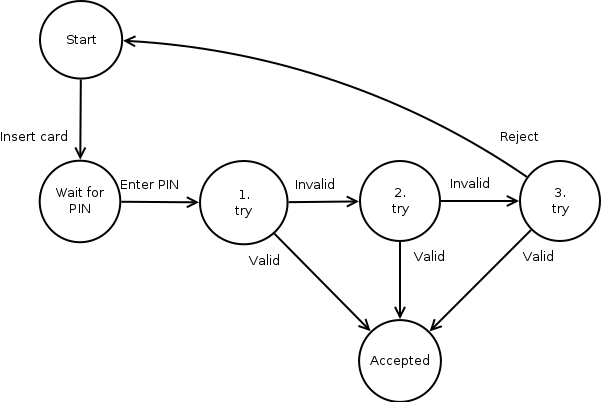
\includegraphics[scale=0.4]{state_transition_diagram.png}
\end{frame}

\begin{frame}
    \frametitle{Test cases}
    Every state and transition criteria.\\
    \begin{enumerate}
        \item Note a starting and end state.
        \item Write a sequence of events that leads to the end state.
        \item Mark each covered state and transition.
        \item Repeat until every state and transition are marked.
    \end{enumerate}
\end{frame}


%------------------------------------------------

\begin{frame}
    \frametitle{The End}

    %\Huge{\centerline{The End}}
    \begin{quote}
        ``Testing shows the presence, not the absence of bugs.''
        \raggedleft{--- Edsger W. Dijkstra}
    \end{quote}
\end{frame}

%----------------------------------------------------------------------------------------

\end{document}

